\documentclass[../main.tex]{subfiles}

\graphicspath{{../images/}}

\begin{document}
\pagestyle{fancy}
\lhead{Lecture 5: 1/30}
\chead{Chapter 4}
\rhead{PHYS 472}

\section*{Chapter 4: Phonons (Lattice Vibrations)}
\addcontentsline{toc}{section}{Chapter 4: Phonons (Lattice Vibrations)}

First starting with the 1D case: evenly spaced atoms we can take the minimum energy energy at the
atom and take the limit as it approaches zero or
\begin{align*}
    \pdv{U}{x} = 0
\end{align*}
the first term is $V \propto x^2$ so we can approximate the potential as
\begin{align*}
    U = \frac{1}{2} U'' x^2 = \frac{1}{2} c x^2
\end{align*}
where $c$ is the spring constant. So we can imagine that the atoms $(u_{s-1}, u_s, u_{s+1})$ are
connected by springs. For 2 coupled springs in series we end up with 2 eigenmodes. But we look at
each pair of atoms and sum up the forces. Using newton's second law we get the force of the $s$ atom 
\begin{align*}
    F_s = c (u_{s+1} - u_s) + c (u_{s-1} - u_s) = c [u_{s+1} + u_{s-1} - 2u_s]
\end{align*}
or as a differential equation
\begin{align*}
    M \dv[2]{u_s}{t} &= c [u_{s+1} + u_{s-1} - 2u_s] \\
    u &= u(\gamma) e^{-i\omega t} \\
    \implies -M \omega^2 u_s &= c [u_{s+1} + u_{s-1} - 2u_s]
\end{align*}
this momentum of the crystal is not conserved but the Hamiltonian can still be written as
\begin{align*}
    H(\gamma) H(\gamma + T)
\end{align*}
where we discretize the translational symmetry, so we can write the periodic part of the atom as
\begin{align*}
    u_s^k = u e^{-ik\gamma \qquad u(\gamma) = u(\gamma + T)}
\end{align*}
where $k = 2\pi/L$ is the wavevector. So we can write the $u_{s-1}$ and $u_{s+1}$ as a translation
of $u_s$:
\begin{align*}
    u_{s-1} &= u e^{-i(s-1)ka} \\
    u_{s+1} &= u e^{i(s+1)ka} \\
    u_s &= u e^{-iska}
\end{align*}
where $a$ is the lattice spacing. subbing this back in:
\begin{align*}
    -M \omega^2 &= c \qt[e^{-ika} + e^{ika} - 2] \\
    \omega^2 &= 2 \frac{c}{M} (1 - \cos(ka))
\end{align*}
using the trig identity for half angles we get 
\begin{align*}
    \omega^2 = \frac{4c}{M} \sin[2](\frac{ka}{2}) \qor
    \omega = 2\sqrt{\frac{c}{M}} \abs{\sin(\frac{ka}{2})}
\end{align*}
where $\omega = ck$ is the dispersion relation where we have boundaries at
$\pm \pi/a$ and max $2\sqrt{c/m}$. The group velocity is
\begin{align*}
    v_g = \pdv{\omega}{k}
\end{align*}
for $k \to 0$ we get the group velocity
\begin{align*}
    v_g = a \sqrt{\frac{c}{M}}
\end{align*}
we also get from the graph of $\omega$ is that the slope at the boundaries are zero. 


\pagebreak
\lhead{Lecture 6: 2/1}

\section*{Chapter 4: cont'd}
\begin{figure} [ht]
    \centering
    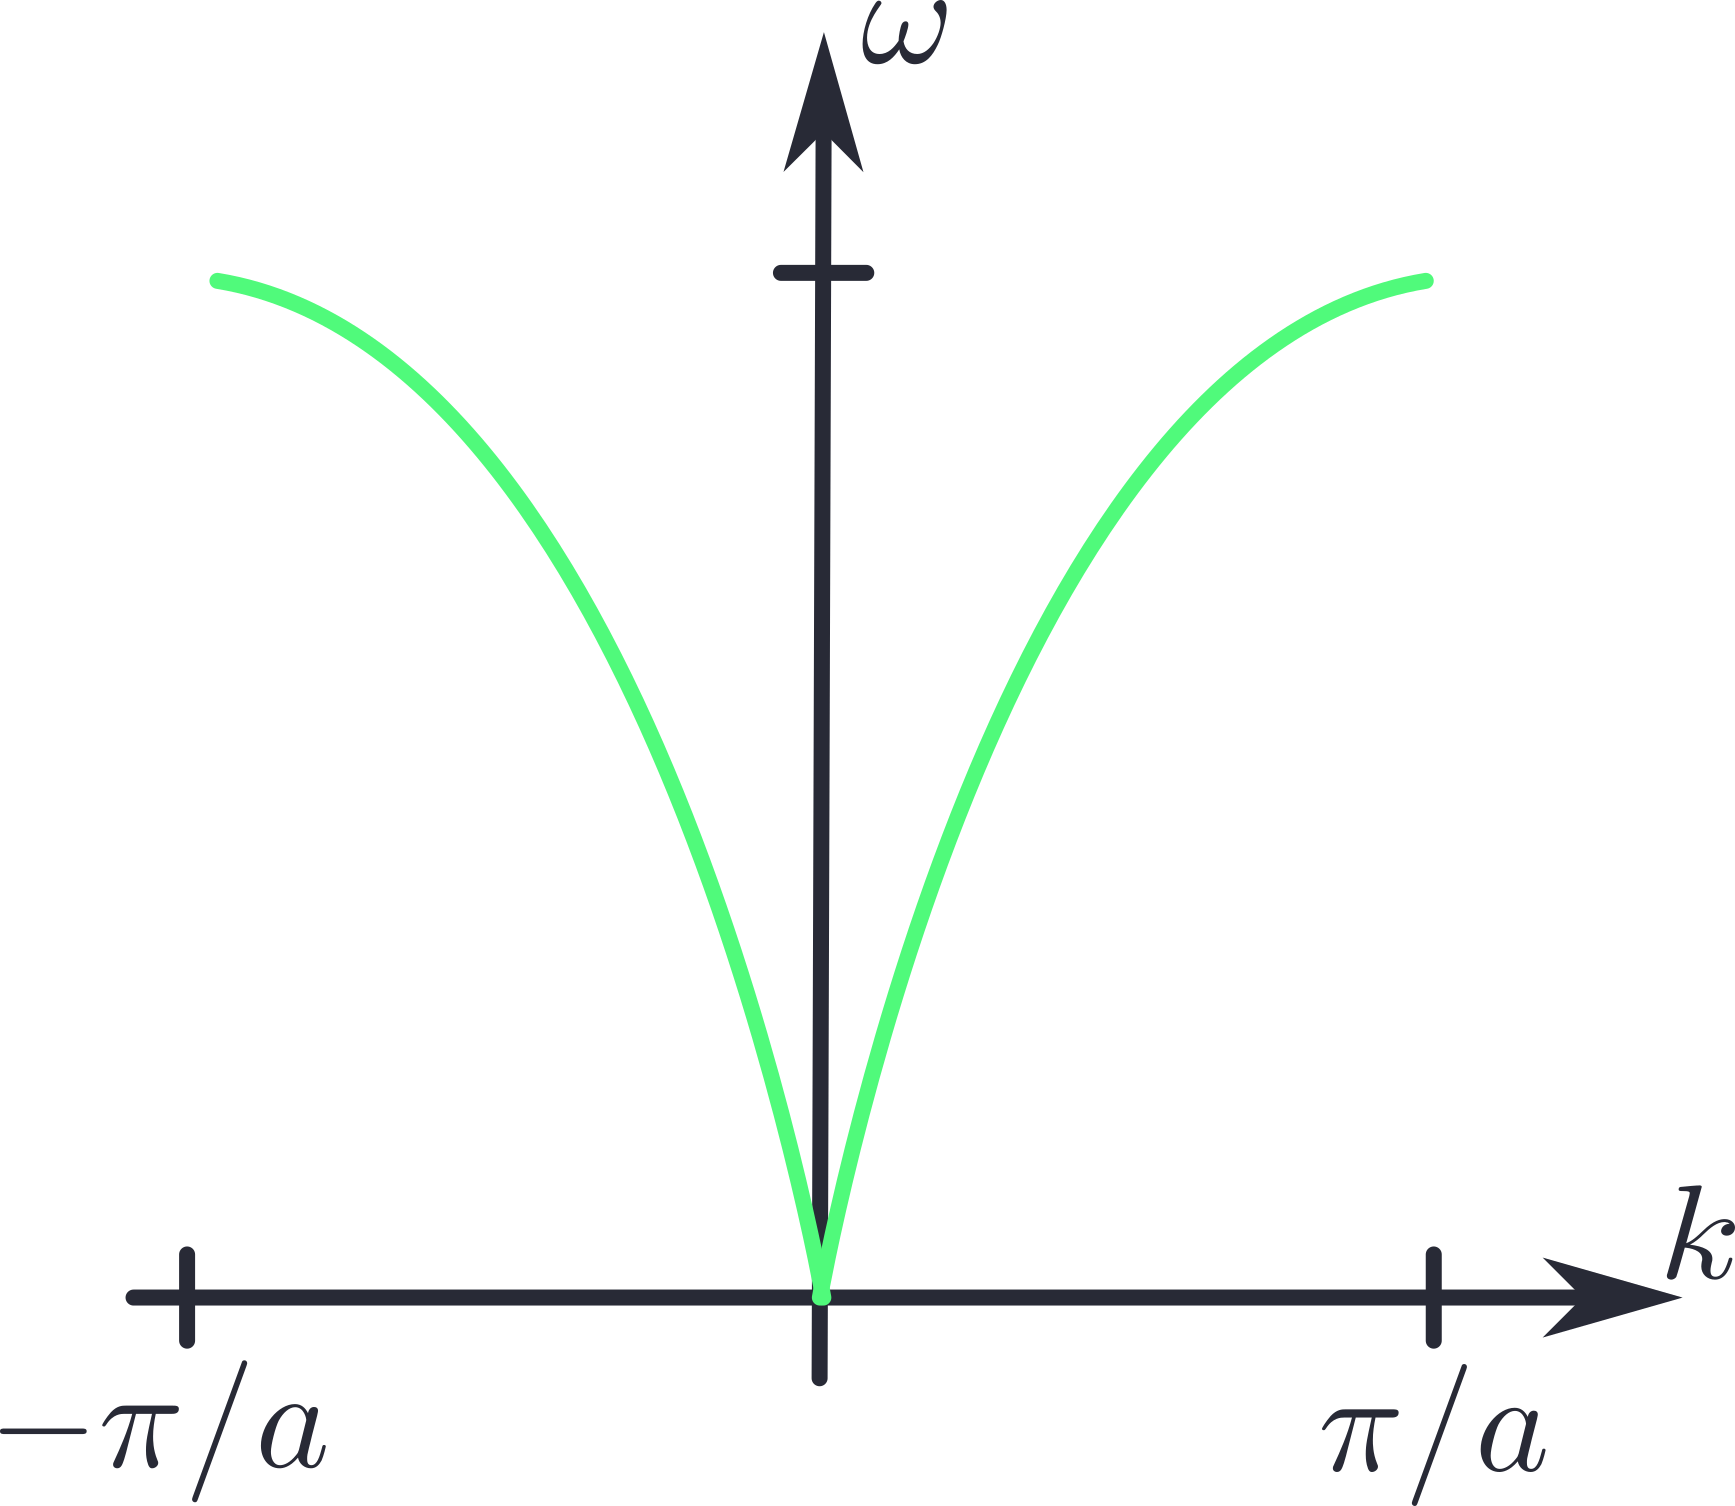
\includegraphics[width=0.4\linewidth]{phonon1.png}
    \caption{Graph of $\omega$ vs $k$}
    \label{fig:5.1}
\end{figure}

Graphing $\omega$ vs $k$ we get the graph in Figure \ref{fig:5.1}. The slope at the boundaries is
zero, and the maximum is $2\sqrt{c/M}$. But as $k \to 0$ we know that $\omega = 0$ and the energy
is also zero. We can imagine the atoms are moving in phase (oscillating in the same direction) and
amplitude. For $\omega = 2\sqrt{c/M}$ we have the atoms moving out of phase (moving in opposite of
their neighbors with equal amplitude). At this point $k = \pi/a$ the potential is
\begin{align*}
    e^{i\pi/a \cdot a} \to e^{i\pi}
\end{align*}

\begin{figure}[ht]
    \centering
    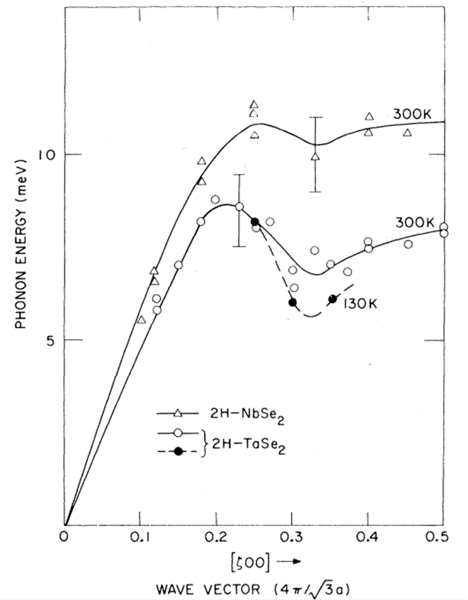
\includegraphics[width=0.4\linewidth]{phonon2.png}
    \caption{Graph of $\omega$ vs $k$ for different material and temperature}
    \label{fig:5.2}
\end{figure}
Figure \ref{fig:5.2} shows the graph of $\omega$ vs $k$ for neutron scattering observed in different
materials and temperatures. We can see that the lower temperature has a low energy mode. 

\paragraph{Aside:} For phonons in low temperature, we see a double well potential, but for high
temperatures, we see negative potential as shown in Figure \ref{fig:5.2}. 

\paragraph{Two atom per unit cell} (primitive basis) For the 1D case again:
\begin{figure}[ht]
    \centering
    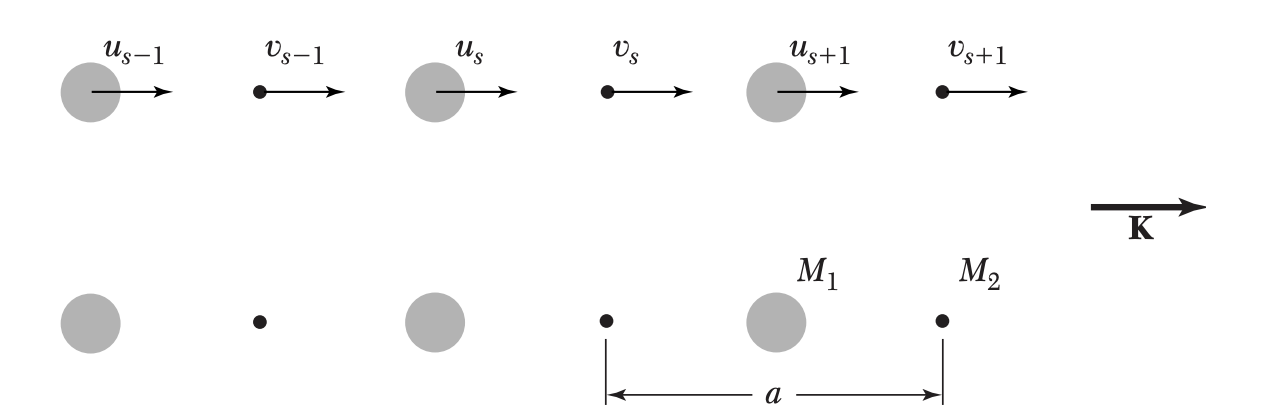
\includegraphics[width=0.8\linewidth]{2basis.png}
    \caption{Two atom per unit cell}
    \label{fig:5.3}
\end{figure}

Using newton's second law
\begin{align*}
    M_1 \ddot{u_s} &= c [v_s + v_{s-1} - 2u_s] \\
    M_2 \ddot{v_s} &= c [u_s + u_{s+1} - 2v_s]
\end{align*}
and the periodic nature of the lattice
\begin{align*}
    u_s &= u e^{iska} e^{-i\omega t} \\
    v_s &= v e^{iska} e^{-i\omega t}
\end{align*}
from substitution we get
\begin{align*}
    -M_1 \omega^2 u &= cv \qt[1 + v e^{-ika}] - 2u \\
    -M_2 \omega^2 v &= cu \qt[1 + u e^{ika}] - 2v
\end{align*}
or in matrix form
\begin{align}
    -\omega^2 \mqty(M_1 & 0 \\ 0 & M_2) \mqty(u \\ v) 
    = c \mqty(-2c & c[1 + e^{-ika}] \\ c[1 + e^{ika}] & -2c) \mqty(u \\ v)
\end{align}
to find the eigenvalues we solve the determinant of the matrix. We can only do this if the matrix is
real (hermitian: complex conjugate is the same as the original). Solving for zero
\begin{align*}
    A = \begin{vmatrix}
        -\omega^2 M_1 + 2c^2 & -c^2(1 + e^{-ika}) \\
        -c^2(1 + e^{ika}) & -\omega^2 M_2 + 2c^2
    \end{vmatrix} \mqty(u \\ v)= 0
\end{align*}
and the determinant of $A$ is
\begin{align*}
    \omega^4 M_1 M_2 - 2c^2 \omega^2 (M_1 + M_2) + 4c^4 + c^2(1 + e^{-ika})(1 + e^{ika}) &= 0 \\
    \omega^4 (M_1 M_2 - 2c^2 (M_1 + M_2) + 4c^4 - c^4[2 + 2 \cos(ka)]) &= 0
\end{align*}
for $k = 0$ we get
\begin{align*}
    M_1 M_2 w^4 - 2c[M_1 + M_2]\omega^2 = 0
\end{align*}
we get the solutions
\begin{align*}
    \omega_o &= 0 \\
    \omega_1 &= \sqrt{\frac{2c(M_1 + M_2)}{M_1 M_2}}
\end{align*}
for $k = \pi/a$ we get
\begin{align*}
    \omega^4 M_1 M_2 - 2c \omega^2(M_1 + M_2) + 4c^4 &= 0
\end{align*}
Physically, the $k=0$ mode there are two solutions, one where all basis move in the same direction,
and the other where each atom moves in the opposing direction. For $k = \pi/a$ we have a solution
where the basis pair move in the opposite direction of its neighbors. For this special case, we know
that the Brillouin zone is half the size of the original zone, so the zone folds in half. 

\paragraph{Phonon modes} For the $k=0$, in the $\omega_o = 0$ case we know that
$\lambda \to \infty$ and it is called an acoustic phonon, but for $\omega_1$ this is an optical 
phonon. This is in the order of meV around the room temperature. For energy of the phonon,
\begin{align*}
    E = \hbar \omega = pc \qand p = \hbar k
\end{align*}
Raman scattering is related to the scattering of light from the optical phonon. The wavelength of
incoming and outgoing light shift by the energy of the phonon.

\paragraph{3D Case:} $N$ atoms per unit cell. We have $3N$ branches of phonons. 3 acoustic and
$3N - 3$ optical phonon.

\paragraph*{Raman Scattering \& Infrared} (THz) $\sim$ 100 meV.
For the 3D case, we have 3 acoustic modes and $3N - 3$ optical modes. FOr the acoustic mode.
\begin{align*}
    k \to 0, \quad \omega \to 0
\end{align*}
and for the optical modes
\begin{align*}
    k \to 0, \quad \omega \to \infty
\end{align*}

\end{document}